\begin{exercises} 
  \item Consider the function $f(x) = 3x + 4$.
  \ba
  	\item Compute $M_4$ for $y=f(x)$ on the interval $[2,5]$.  Be sure to clearly identify the value of $\triangle x$, as well as the locations of $x_0, x_1, \ldots, x_4$.  Include a careful sketch of the function and the corresponding rectangles being used in the sum.
	\item Use a familiar geometric formula to determine the exact value of the area of the region bounded by $y = f(x)$ and the $x$-axis on $[2,5]$.
	\item Explain why the values you computed in (a) and (b) turn out to be the same.  Will this be true if we use a number different than $n = 4$ and compute $M_n$?  Will $L_4$ or $R_4$ have the same value as the exact area of the region found in (b)?
	\item Describe the collection of functions $g$ for which it will always be the case that $M_n$, regardless of the value of $n$, gives the exact net signed area bounded between the function $g$ and the $x$-axis on the interval $[a,b]$.
  \ea	
  \item Let $S$ be the sum given by
  $$S = ((1.4)^2 + 1) \cdot 0.4 + ((1.8)^2 + 1) \cdot 0.4 + ((2.2)^2 + 1) \cdot 0.4 + ((2.6)^2 + 1) \cdot 0.4 +((3.0)^2 + 1) \cdot 0.4.$$
  	\ba
		\item Assume that $S$ is a right Riemann sum.  For what function $f$ and what interval $[a,b]$ is $S$ an approximation of the area under $f$ and above the $x$-axis on $[a,b]$?  Why?
		\item How does your answer to (a) change if $S$ is a left Riemann sum?  a middle Riemann sum?
		\item Suppose that $S$ really is a right Riemann sum.  What is geometric quantity does $S$ approximate?
		\item Use sigma notation to write a new sum $R$ that is the right Riemann sum for the same function, but that uses twice as many subintervals as $S$.
	\ea
	\item A car traveling along a straight road is braking and its velocity is measured at several different points in time, as given in the following table.
\begin{center}
\begin{tabular}{|l|c|c|c|c|c|c|c|}
\hline
seconds, $t$ & 0 & 0.3 & 0.6 & 0.9 & 1.2 & 1.5 & 1.8 \\
\hline
Velocity in ft/sec, $v(t)$ & 100 & 88 & 74 & 59 & 40 & 19 & 0 \\
\hline
\end{tabular}
\end{center}
\ba
	\item Plot the given data on a set of axes with time on the horizontal axis and the velocity on the vertical axis.
	\item Estimate the total distance traveled during the car the time brakes using a middle Riemann sum with 3 subintervals.
	\item Estimate the total distance traveled on $[0,1.8]$ by computing $L_6$, $R_6$, and $\frac{1}{2}(L_6 + R_6)$.
	\item Assuming that $v(t)$ is always decreasing on $[0,1.8]$, what is the maximum possible distance the car traveled before it stopped?  Why?
\ea
	\item The rate at which pollution escapes a scrubbing process at a manufacturing plant increases over time as filters and other technologies become less effective.  For this particular example, assume that the rate of pollution (in tons per week) is given by the function $r$ that is pictured in Figure~\ref{F:4.2.Ez4}.
\begin{figure}[h]
\begin{center}
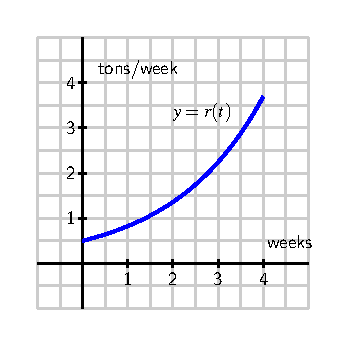
\includegraphics{figures/4_2_Ez4.eps}
\caption{The rate, $r(t)$, of pollution in tons per week.} \label{F:4.2.Ez4}
\end{center}
\end{figure} 
	\ba
		\item Use the graph to estimate the value of $M_4$ on the interval $[0,4]$.
		\item What is the meaning of $M_4$ in terms of the pollution discharged by the plant?
		\item Suppose that $r(t) = 0.5 e^{0.5t}$.  Use this formula for $r$ to compute $L_5$ on $[0,4]$.  
		\item Determine an upper bound on the total amount of pollution that can escape the plant during the pictured four week time period that is accurate within an error of at most one ton of pollution.
	\ea
\end{exercises}
\afterexercises
